% \documentclass[a4paper,twoside,twocolumn,10pt]{article}
\documentclass[a4paper,twoside,twocolumn,10pt]{jarticle}     %pLaTeX2e仕様(platex.exeの場合)
\usepackage{abstract} % Style for abstracts in Dept. CSIS, OPU
%\usepackage{abstract4past} % Style for abstracts for the past curriculum

%%%%%%%%%% Designate packages you need %%%%%%%%%%
% \usepackage{graphicx} % Enhanced support for graphics
\usepackage[dvipdfm]{graphicx}
\usepackage{url} % Verbatim with URL-sensitive line breaks

%%%%%%%%%% Parameters that should be customized %%%%%%%%%%
% Language (1 = Japanese, 2 = English)
\setlang{1}
% Bachelor or Master (1 = Bachelor, 2 = Master)
\setborm{1}
% Fiscal year
\setfy{2020}
% Group number
\setgnum{1}
% Presentation order
\setorder{6}
% Increase page number (optional)
%% \pplus{1}

\title{遺伝的アルゴリズムによる機械学習における\\疑似ラベル生成手法の提案}
\author{細川 岳大}
%\ordering{6}[B]  %?²?_?ÍB?C?C?_?ÍM
\begin{document}
\maketitle
\small
\section{はじめに}
近年,ラベル付きデータ生成に伴うコストの観点から分類問題において半教師あり学習
 (Semi-Supervised Learning: SSL)と呼ばれる
学習データ全体のうち一部にのみラベル付けされた状態で学習を行う手法が
盛んに研究されている.
しかし,当然のことながら各ラベルに対するデータ数が少ないほど精度が
安定しなくなるという問題も報告されている.
一方で,ラベルなしデータへのラベル付けタスクは一種の組合せ最適化問題と考えることができる.

そこで本研究では,組合せ最適化遺伝的アルゴリズムを用いて
データにラベルを付与することでラベル付きデータが少ない場合における半教師あり学習の頑健
性を高める手法を提案する.
\section{要素技術}
\subsection{Contrastive Learning}
Contrastive Learning (CL) とは,特徴表現を獲得するための
自己教師あり学習のひとつである.
一つの画像から得られる特徴表現が画像変換によって
画像の持つ意味が大きく変わらない変形を獲得することができる.
\subsection{SimCLR}
Simple framework for Contrastive Learning of visual Representation(SimCLR)\cite{chen2020simple}は SSL の一つであり,
 CL により特徴抽出器を学習したうえで,少量のラベル付きデータによる Fine tuning によって分類器を獲得する手法である.

\subsection{遺伝的アルゴリズム}
遺伝的アルゴリズム (Genetic Algorithm: GA) は生物の進化を模倣した最適解探索アルゴリズムである.
選択,交叉,突然変異の3つの操作によって最適解を探索することができる.
\section{提案手法}
本研究では, CIFAR-10 においてラベルありとラベルなしに分割し,ラベルなしデータの一部に対するラベルを GA によって探索する.
GA の個体について各遺伝子はラベルデータのいずれかの整数値とし,取り出されたラベルなしデータに対する疑似ラベルとする.
以下に提案手法の概要を示す.
\begin{enumerate}
	\item CL によって特徴抽出器を学習する.
	\item GA の個体と対応するデータを学習データとし, Fine tuning を行い,ラベル付きデータに対する識別率
	を適応度として GA の探索を行う.
	\item 探索された個体とラベル付きデータを学習データとし, Fine tuning を行い,テストデータを識別する.
\end{enumerate}
\section{数値実験}
\subsection{実験方法}
データセットとして10クラス識別問題である CIFAR-10 を用いた.
学習に50000件,テストに10000件をそれぞれ使用し,ラベル付きデータ及びランダムに選ばれた
疑似ラベルを付与する対象であるラベルなしデータはどちらも学習データから選んだ.
CL の学習について,特徴抽出器には Resnet-18 を用い,学習データ50000件を,500 epoch 学習した.
また分類器は MLP を使用した.
GA の適応度計算については,30 epoch 学習した.
\subsection{結果と考察}
\begin{figure}[t]
	\begin{center}
		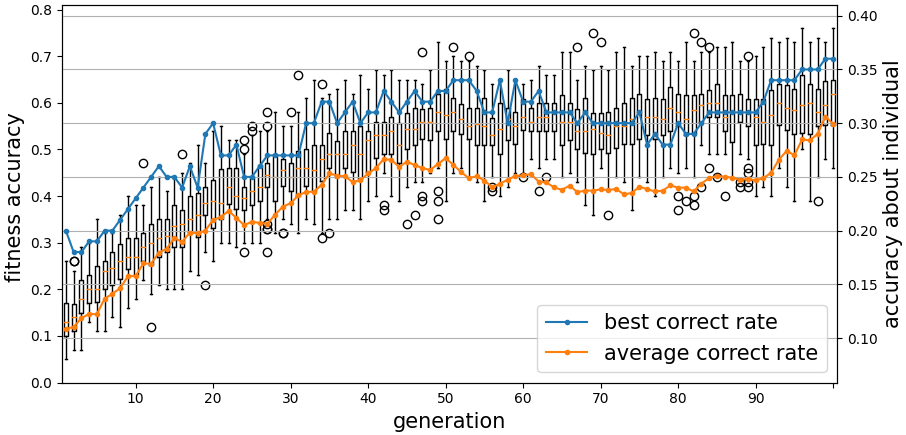
\includegraphics[height=55mm,width=90mm]{graph.png}
		\caption{各世代に対する適応度と疑似ラベルの正答率\label{fig:ex1}}
	\end{center}
\end{figure}
表\ref{tb:ex1}と図\ref{fig:ex1}に結果の一例を示す.また,図\ref{fig:ex1}の横軸に世代を,縦軸は箱ひげ図が適応度,折れ線グラフが各個体の疑似ラベルに対する正解ラベルの割合である. 提案手法が最も低い精度となった一方で,GA の探索については進んでいるといえ,
疑似ラベルに対する真の正答率は 37\%まで上がっていることが確認できた.

考察として GA の探索において今回の設定では多様性を保つことができず,局所解に陥ってしまったのではないかと考えられる.また,ラベルの多くが誤ラベルのため train\_accuracy が学習において 80\%以上にならず各個体に対しての正確な適応度が求められなかった可能性がある.
\
\begin{table}[h]
	\centering
	\caption{テスト識別率結果\label{tb:ex1}}
	\scalebox{0.8}{
		\begin{tabular}{|c|c|} \hline
			\bf 生成ラベル&\bf テスト識別率\\ \hline\hline
			baseline モデルによる疑似ラベル&0.784\\ \hline
			提案手法による疑似ラベル&0.674\\ \hline\hline
			正解ラベル&0.822\\ \hline\hline
			baseline (ラベル付きデータのみ)&0.772\\ \hline
		\end{tabular}
	}
\end{table}

\section{まとめと今後の課題}
本研究では,GA によるラベルなしデータに対する疑似ラベルの生成手法を提案した.

今後の課題として,GA の拡張手法や適応度の計算方法を工夫することでより
良質な疑似ラベルを生成し識別率向上を目指すことが挙げられる.

\bibliographystyle{unsrt}
\bibliography{sa}

\end{document}

